\section{Specific Model of Bovine Viral Diarrhea}
\label{chap:bvdModel}
The basic SIR-Model as it is discussed in chapter \ref{chap:generalModeling} is unfortunately not sufficient to describe a complex illness like BVD. This section therefore tries to give a brief introduction to the disease and how it can be modeled.

Since this is a thesis that is supposed to focus on the theoretical and mathematical description and interpretation of the phenomena observed around BVD (and it's Virus BVDV), the introduction to the biological phenomena will be rather short. For this purpose the author relies on \citep{LIN03}, which is a paper that has been cited a lot and which has been published $14\,\text{years}$ earlier to this thesis.

\subsection{BVD Basics}\label{chap:bvdBasics}
Bovine Viral Diarrhea is a virus infection that leads to various symptoms depending on the status of the cow. Most of the effects, which will be neglected in the modeling of the disease, will also be neglected in this explanation. \citep{openagrar_mods_00019481} gives a very brief overview on the disease as such, \citep{LIN03} describes the biological influence of the disease on the animals very detailed.

\paragraph{Non-Pregnant Cows} If a bovine becomes infected while not being pregnant, the numbers of white blood cells and thrombocytes decrease. According to \citep{LIN03} this can even lead to a lessened semen quality in infected bulls where the virus may even persist in the testicles. Furthermore the virus can be detected $4 \text{ to } 10\,\text{days}$ after infection in most secretes and \glqq clinical symptoms such as fever, post infection, inappetence and mucosal lesions\grqq. The symptom, that gave this disease its name, diarrhea, as well as coughing are mostly seen in calves, but it is not entirely clear, if this might be due to a secondary infection that is caused by the immune suppressive effect of the loss of white blood cells and thrombocytes.
A recovered cow with a normally working immune system will be immune to BVDV for the rest of its life and its calves will also be protected by the maternal antibodies in the cow's milk for the first $4-6\, \text{months}$ of their lives. If calves get vaccinated while being protected by maternal antibodies, the vaccination will not protect them from the disease. However the majority of farmers mixes their colostrum \citep{personalCom}. This can lead to a bigger group of immune calves, but it could possibly dilute the antibody levels below the threshold where it actually creates an immune response.

\paragraph{Pregnant Cows}
For the mother the virus will have little implications, but the unborn calf can suffer a various number of complications. The mother can become infertile, while the calve can die, have malformations, be retarded, weak or stillborn, but most importantly some calves could become persistently infected (PIs). These calves will be infectious during their whole life time and produce high amounts of the virus. Their body does not detect the virus as harmful and therefore does not build up antibodies \citep{personalCom}. Calves of PIs are always PIs too. PIs have a much shorter life span, especially because they can suffer secondary illnesses such as mucosal disease which triggers diarrhea and can be survived by chronic cases for up to $18\,\text{months}$.

\subsection{Compartmental Model}
Without further conclusions the full system of differential equations shall be presented here for the sake of completeness. Figure \ref{fig:bvdDia} shows the different health statuses a bovine can acquire and the different transition rates as they are used in the equations (\ref{eq:m1}) to (\ref{eq:p1}) adopted with slight modifications from \ref{BAS16}
The alert reader may have noticed that BVD as it is discussed in chapter \ref{chap:bvdBasics} could be described with a SIR-Model with slight modifications. 
\begin{figure}[htbp]
\centering
\noindent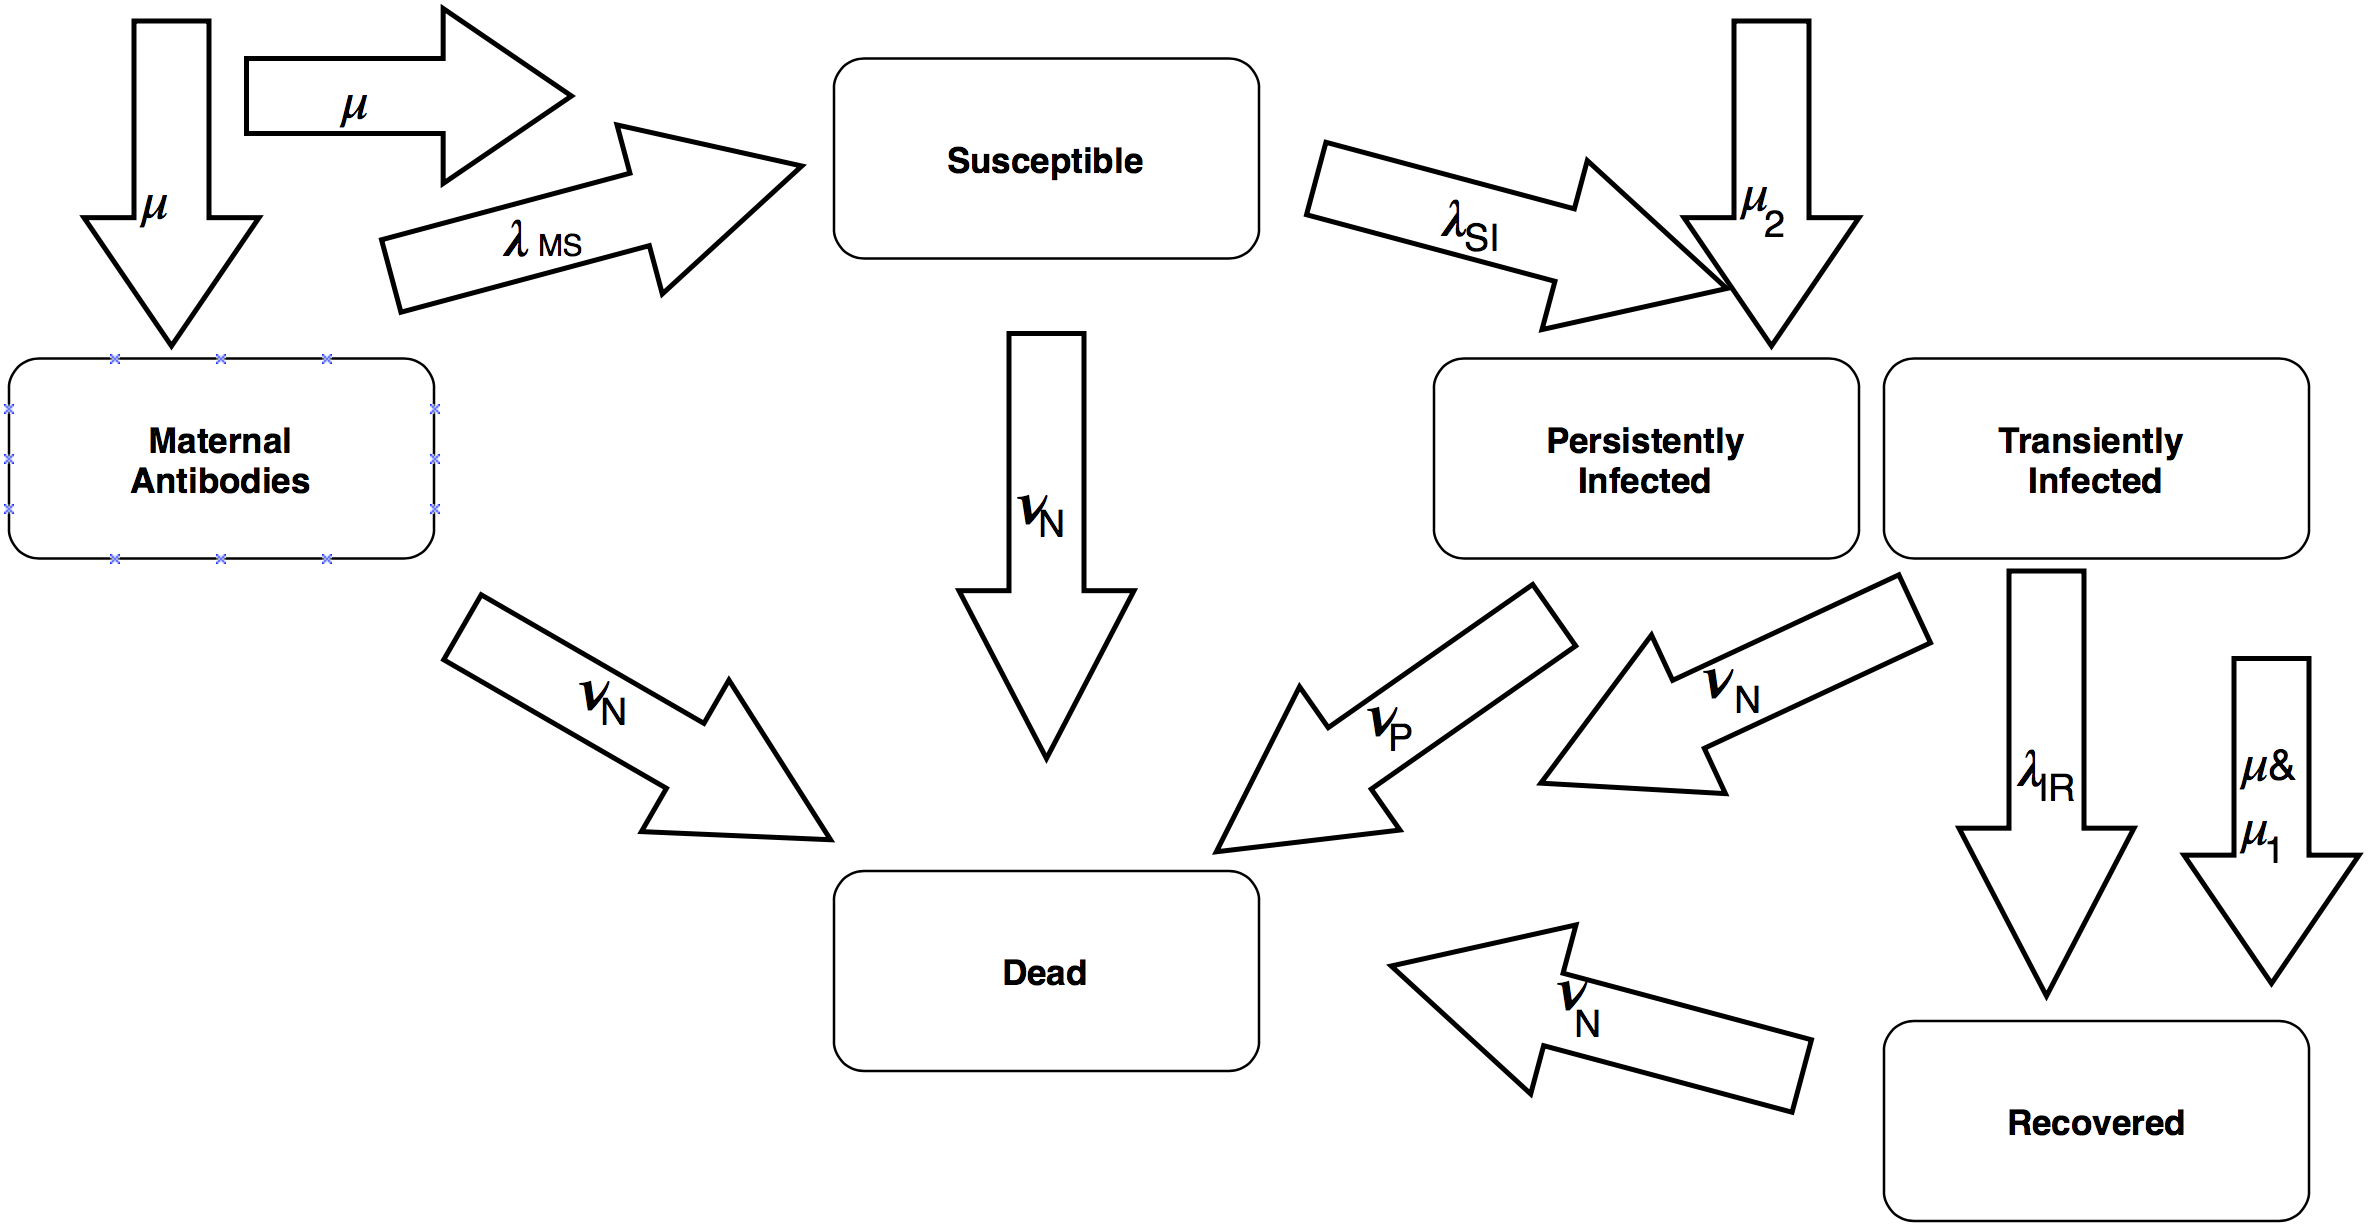
\includegraphics[width=\linewidth,height=\textheight,
keepaspectratio]{bvdDia.png} \caption[BVD Disease Spread Illustration]{This graphic shows how the different transition rate influence the different states. All transition rates called $\mu$ require a birth event, all rates $\nu$ a death, all rates $\lambda$ imply a change in the health state of an individual.}
\label{fig:bvdDia}
\end{figure}
In addition to the model we add two new groups: the group of calves protected by maternal antibodies in their milk, the MAs, the group of persistently infected cows, the PIs, and in order to make it easier to differentiate between the two groups of infected, the group normally marked as I will be called TI\footnote{In order to improve the readability of of all equations PIs will be marked as $P$, MAs as $M$ and TIs as $I$.}.
With a death rate of non PIs $\nu_\text{N}$, a death rate of PIs $\nu_\text{P}$, a general birth rate $\mu$ and birth rates for recovered $\mu_1$ and PIs $\mu_2$ after an infected met a susceptible at the right point in time we get:

\begin{eqnarray}
\dot{M}  =& \mu R-\lambda_\text{MS} M -\nu_\text{N} M & \label{eq:m1}\\
\dot{S}  =& \lambda_\text{MS} M - \lambda_\text{SI}SI-\lambda_\text{SP} SP &-\nu_\text{N} S + \mu S \\
\dot{I}  =& \beta_\text{SI}SI+\beta_\text{SP} SP - \lambda_\text{IR} I &- \nu_\text{N} I \label{eq:idotbvd} \\
\dot{R}  =& \lambda_\text{IR}I - \nu_\text{N} R +\mu_1S(t-\tau_1)I(t-\tau_1) &+\mu_1S(t-\tau_1)P(t-\tau_1) \\ 
\dot{P}  =&  \mu P -\nu_\text{P}P + \mu_2S(t-\tau_2)I(t-\tau_2) &+ \mu_2S(t-\tau_2)P(t-\tau_2) \label{eq:p1}
\end{eqnarray}
following \citep{BAS16} with the infection probabilities when a PI or a TI meet a susceptible $\beta_\text{PI}$ and $\beta_\text{TI}$. The time delays $(t-\tau_1)$ and $(t-\tau_2)$ are visualized in figure \ref{fig:infectionTimeScale}. For simplification purposes it is assumed, that the infections during a pregnancy, leading to recovered or persistently infected calves, take place at a fixed time before birth. Usually they would need to be expressed by integrals over a time frame. The different time windows of the pregnancy with the corresponding probabilities of all different results are presented in \ref{appendix:diseasesistributions}. Equation (\ref{eq:idotbvd}) can be rewritten like:
\begin{eqnarray}
\dot{I}  =& \lambda_\text{SIges}S - \lambda_\text{IR}&I - \nu_\text{N} I, \text{ with} \\
\lambda_\text{SIges} =& \beta_\text{SI} I+ \beta_\text{PI} P.& \label{eq:vie04start}
\end{eqnarray}
This system of nonlinear differential equations can not be solved easily and assume a well mixed population and have all the negative characteristics of such description described in \ref{chap:agentBasedModelBasics}. Still it can be used to get some insights about the disease as such. For example the idea of the basic reproduction number $R_0=\lambda_\text{SI} / \lambda_\text{IR}$ from chapter \ref{chap:sirBasic} could be used. An equivalent of the basic reproduction number is not trivial to obtain, but still putting some thought into it is worthwhile. 
Because PIs do not recover, the basic reproduction number will always be big compared to a standard SIR model, this part would go to infinity. This will lead to a more stable population of persistently infected when compared to infecteds in a standard SIR model.

\begin{figure}[htbp]
\centering
\noindent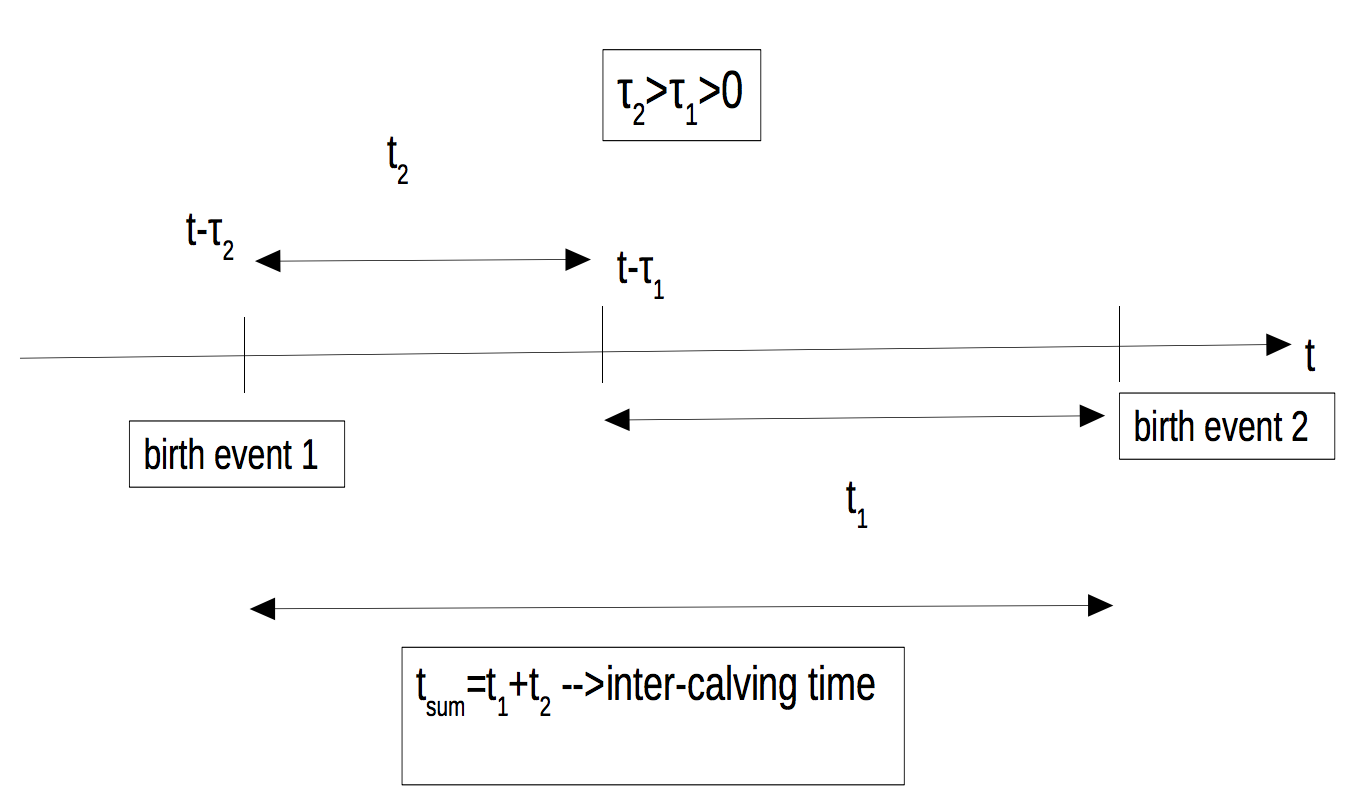
\includegraphics[width=\linewidth,height=\textheight,
keepaspectratio]{infectionTimeScale.png} \caption[Visualization of time delays in the mean field model]{This picture illustrates the time delays in the mean field equations given above.}
\label{fig:infectionTimeScale}
\end{figure}
